\documentclass[paper=a4, fontsize=11pt]{scrartcl} % KOMA-article class

%-------------------------------------------------
%   THEMES, PACKAGES, CUSTOM COMMANDS
%-------------------------------------------------
\usepackage{blindtext}
\usepackage[english]{babel}                             % English language/hyphenation
\usepackage[protrusion=true,expansion=true]{microtype}  % Better typography
\usepackage{amsmath,amsfonts,amsthm}                    % Math packages
\usepackage[pdftex]{graphicx}                           % Enable pdflatex
\usepackage[export]{adjustbox}
\usepackage[svgnames]{xcolor}                           % Enabling colors by their 'svgnames'
\usepackage[hang, small,labelfont=bf,up,textfont=it,up]{caption} % Custom captions under/above floats
\usepackage{subcaption}
\usepackage{caption}
\usepackage{epstopdf}       % Converts .eps to .pdf
%\usepackage{subfig}         % Subfigures
\usepackage{booktabs}       % Nicer tables
\usepackage{fix-cm}         % Custom fontsizes
\usepackage{listings}
\usepackage{soul}
\usepackage{float}

\usepackage{hyperref}

\usepackage[foot=30pt,margin=1in]{geometry}

% Custom sectioning (sectsty package)
\usepackage{sectsty}
\allsectionsfont{
    \usefont{OT1}{phv}{b}{n}    % bch-b-n: CharterBT-Bold font
}
\sectionfont{
    \usefont{OT1}{phv}{b}{n}
}

% Custom colors
\definecolor{brsugrey}{rgb}{0.9, 0.9, 0.9}
\definecolor{brsublue}{rgb}{0, 0.594, 0.949}

%
\newcommand{\upperRomannumeral}[1]{\uppercase\expandafter{\romannumeral#1}}

% Creating an initial of the very first character of the content
\usepackage{lettrine}
\newcommand{\initial}[1]{%
    \lettrine[lines=3,lhang=0.3,nindent=0em]{
        \color{brsublue}
        {\textsf{#1}}}{}}

%-------------------------------------------------
%   COMMON INFO
%-------------------------------------------------
\newcommand{\hmwkTitle}{Bayesian Networks Homework}
\newcommand{\hmwkDueDate}{Due date: November 30, 2016}
\newcommand{\hmwkClass}{Advanced Mathematics for Robotics and Control}
\newcommand{\hmwkClassShort}{AMRC WS2016}
\newcommand{\hmwkAuthorFullName}{Minh H. Nguyen}
\newcommand{\hmwkAuthorLastName}{Nguyen}
\newcommand{\hmwkAuthorEmail}{minh.nguyen@smail.inf.h-brs.de}
\newcommand{\hmwkAuthorInstitute}{BRS University of Applied Sciences}

%-------------------------------------------------
%   HEADERS & FOOTERS
%-------------------------------------------------
\usepackage{fancyhdr}
\pagestyle{fancy}
\usepackage{lastpage}
% Header (empty)
\lhead{}
\chead{}
\rhead{}
% Footer (you may change this to your own needs)
\lfoot{\footnotesize
    \texttt{\hmwkClassShort} ~
    \textbullet ~ \hmwkAuthorLastName ~
    \textbullet ~ \hmwkTitle}
\cfoot{}
\rfoot{\footnotesize page \thepage\ of \pageref{LastPage}}  % "Page 1 of 2"
\renewcommand{\headrulewidth}{0.0pt}
\renewcommand{\footrulewidth}{0.4pt}

%-------------------------------------------------
%   TITLE & AUTHOR
%-------------------------------------------------
\usepackage{titling}

\newcommand{\HorRule}{\color{brsublue}% Creating a horizontal rule
    \rule{\linewidth}{1pt}%
    \color{black}
}

% Title
\pretitle{
    \vspace{-30pt}
    \begin{flushleft}
        \HorRule
        \fontsize{19}{19} \usefont{OT1}{phv}{b}{n} \color{gray} \selectfont
}
\title{\hmwkClass \\
       \hmwkTitle}
\posttitle{
    \par
    \end{flushleft}
    \vskip 0.5em
}

% Author
\preauthor{
    \begin{flushleft}
        \large \lineskip 0.25em
        \usefont{OT1}{phv}{b}{sl} \color{brsublue}}

\author{\hmwkAuthorFullName}

\postauthor{
        \footnotesize
        \usefont{OT1}{phv}{m}{sl} \color{Black}
        \\\hmwkAuthorInstitute
        \\\hmwkAuthorEmail
        \par
    \end{flushleft}
    \HorRule}

% Date
\date{\hmwkDueDate}

%-------------------------------------------------
%   BEGIN
%-------------------------------------------------
\begin{document}
    \maketitle
    \thispagestyle{fancy} % Enabling the custom headers/footers for the first page

\section*{Exercise 3.11}

    \begin{figure}[H]
        \centering
        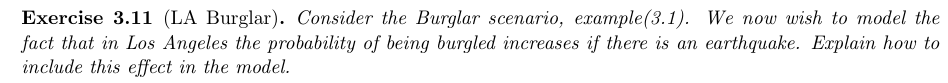
\includegraphics[width=\linewidth]{../images/barber_ex3-11_problem.png}
    \end{figure}

    \begin{figure}[H]
        \centering
        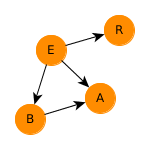
\includegraphics[width=0.3\linewidth]{../images/barber_ex3-11.png}
        \caption{BN for Burglar problem, where B represents burglary, represents earthquake, A represents Alarm, and R represents radio reporting earthquake}
    \end{figure}

    Adding connection from E to B allows representing the relation that an earthquake happening increases the chance of a burglary happing.

\section*{Exercise 3.15}

    \begin{figure}[H]
        \centering
        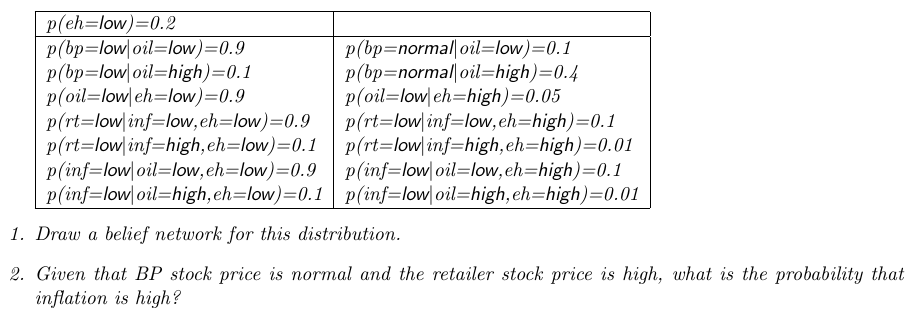
\includegraphics[width=\linewidth]{../images/barber_ex3-15_problem.png}
    \end{figure}

    \subsection*{Belief network}
        \begin{figure}[H]
            \centering
            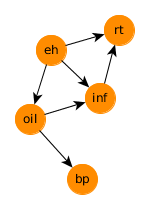
\includegraphics[width=0.3\linewidth]{../images/barber_ex3-15.png}
        \end{figure}

    \subsection*{Probability of inflation}
    \begin{eqnarray}
    p(inf=high | bp=normal) & = &\frac{p(inf=high, bp=normal)}{p(bp=normal)} \\
    p(inf=high, bp=normal) & = & \sum_{eh,oil,rt}p(bp=normal,eh,inf=high,oil,rt) % \sum_{eh}\sum_{oil}\sum_{rt} 
    \end{eqnarray}
    \begin{eqnarray}
    (2) = & \sum_{eh,oil,rt} p(eh) p(oil|eh) p(inf=high | eh, oil) p(rt | eh, inf=high) p(bp=normal|oil) \\
        = & \sum_{eh,oil,rt} p(inf=high | eh, oil) p(rt | eh, inf=high) p(bp=normal|oil)\\
        = & \sum_{eh,oil} p(inf=high | eh, oil) p(bp=normal|oil) \sum_{rt} p(rt | eh, inf=high) p(eh)
    \end{eqnarray}
    \begin{eqnarray}
    p(bp=normal) & = & \sum_{eh,inf,oil,rt}p(bp=normal,eh,inf,oil,rt) \\
    & = & \sum_{eh,inf,oil,rt} p(eh) p(oil|eh) p(inf | eh, oil) p(rt | eh, inf) p(bp=normal|oil) \\
    & = & p(bp=normal | oil)p(oil | eh)p(eh)
    \end{eqnarray}

\section*{Exercise 3.18}

    \begin{figure}[H]
        \centering
        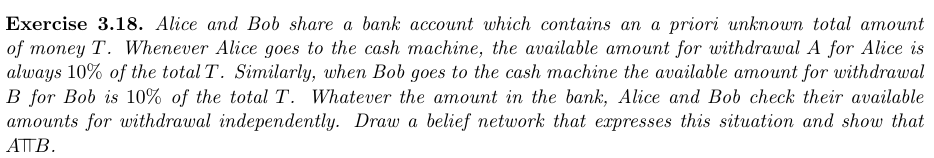
\includegraphics[width=\linewidth]{../images/barber_ex3-18_problem.png}
    \end{figure}

    \begin{figure}[H]
        \centering
        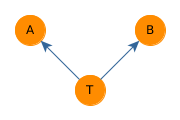
\includegraphics[width=0.5\linewidth]{../images/barber_ex3-18.png}
    \end{figure}

    From definition 3.3, A and B are independent conditioned on T.

%\begin{thebibliography}{9}
%    \bibitem{Thrun}
%    S. Thrun et al., “Velocity Motion Model,” in Probabilistic Robotics, ch. 5, pp. 121–132, Cambridge,
%    MA: The MIT Press, 2006.
%\end{thebibliography}
\end{document}
